% Hardness bounds for Max-k-Cut, 3 <= k <= 24: the quantity 1 - (hardness factor), log scale.
% Needs \usepackage{pgfplots} and \pgfplotsset{compat=1.18} in the preamble (both are in main.tex).
% Legend uses \ref{thm:main45} and \ref{thm:perfect} (Theorems 1.2 and 1.3 of main.tex).
% Coordinates computed exactly (Python fractions), written with 6 significant digits:
%   Thm 1.2:  2/Gamma_L,                    Gamma_L = 29 + 18L + 3 binom(L,2),  L = k-3
%   Thm 1.3:  3/(51 + 34L + 3 binom(L,2)),  k >= 4
%   [AOTW14]: 1/(17(k+c_k)+c_k), c_k = k mod 3, for k >= 4;  1/17 for k = 3
%   [NRT25]:  1 - 0.98708 = 0.01292 at k = 4
\begingroup
%
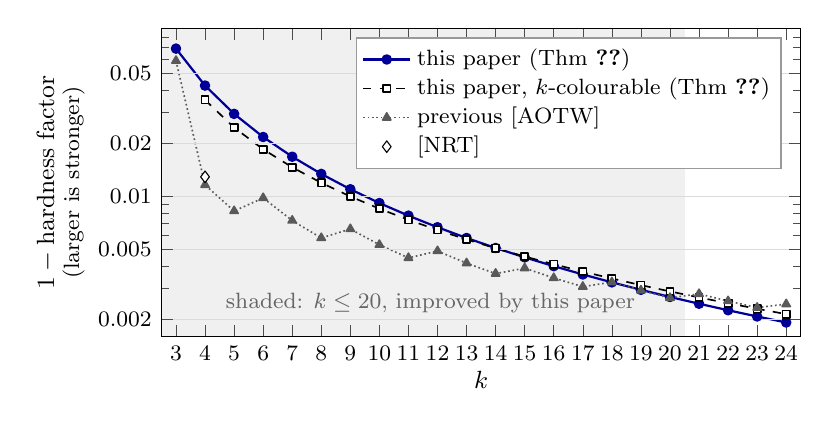
\begin{tikzpicture}
\begin{axis}[
  width=0.8\textwidth, height=5.5cm,
  scale only axis=false,
  xmin=2.5, xmax=24.5,
  ymode=log, ymin=0.0016, ymax=0.09,
  xtick={3,...,24},
  ytick={0.002,0.005,0.01,0.02,0.05},
  yticklabels={$0.002$,$0.005$,$0.01$,$0.02$,$0.05$},
  minor ytick={0.003,0.004,0.006,0.007,0.008,0.009,0.03,0.04,0.06,0.07,0.08,0.09},
  ymajorgrids, yminorgrids=false,
  major grid style={black!14,line width=0.3pt},
  tick label style={font=\footnotesize},
  tick style={black!70},
  xlabel={$k$}, xlabel style={font=\small,yshift=3pt},
  ylabel={$1-{}$hardness factor\\[-2pt]{\footnotesize(larger is stronger)}},
  ylabel style={font=\small,align=center,yshift=-2pt},
  axis on top,
  legend cell align=left,
  legend pos=north east,
  legend style={font=\footnotesize,draw=black!40,fill=white,inner sep=2pt,
                row sep=-1pt,line width=0.4pt},
  every axis plot/.append style={line join=round},
]
% range of k in which this paper improves the previous bounds
\fill[black!6] (axis cs:2.5,0.0016) rectangle (axis cs:20.5,0.09);
\node[font=\footnotesize,text=black!60,anchor=south west,inner sep=0pt]
  at (axis cs:4.7,0.00218) {shaded: $k\le 20$, improved by this paper};
% (1) Theorem 1.2
\addplot[blue!60!black, line width=0.8pt, mark=*, mark size=1.5pt,
         mark options={solid,fill=blue!60!black}]
  coordinates {(3,0.0689655) (4,0.0425532) (5,0.0294118) (6,0.0217391) (7,0.0168067)
   (8,0.0134228) (9,0.010989) (10,0.00917431) (11,0.0077821) (12,0.00668896)
   (13,0.00581395) (14,0.00510204) (15,0.00451467) (16,0.00402414) (17,0.00361011)
   (18,0.00325733) (19,0.00295421) (20,0.00269179) (21,0.00246305) (22,0.00226244)
   (23,0.00208551) (24,0.00192864)};
\addlegendentry{this paper (Thm~\ref{thm:main45})}
% (2) Theorem 1.3
\addplot[black, line width=0.6pt, dashed, mark=square*, mark size=1.3pt,
         mark options={solid,fill=white}]
  coordinates {(4,0.0352941) (5,0.0245902) (6,0.0185185) (7,0.0146341) (8,0.0119522)
   (9,0.01) (10,0.00852273) (11,0.00737101) (12,0.00645161) (13,0.00570342)
   (14,0.00508475) (15,0.00456621) (16,0.00412655) (17,0.00375) (18,0.00342466)
   (19,0.00314136) (20,0.00289296) (21,0.0026738) (22,0.00247934) (23,0.00230592)
   (24,0.00215054)};
\addlegendentry{this paper, $k$-colourable (Thm~\ref{thm:perfect})}
% (3) previous bound of [AOTW14]
\addplot[black!65, line width=0.6pt, densely dotted, mark=triangle*, mark size=1.7pt,
         mark options={solid,fill=black!65}]
  coordinates {(3,0.0588235) (4,0.0116279) (5,0.00826446) (6,0.00980392) (7,0.00729927)
   (8,0.00581395) (9,0.00653595) (10,0.00531915) (11,0.0044843) (12,0.00490196)
   (13,0.0041841) (14,0.00364964) (15,0.00392157) (16,0.00344828) (17,0.00307692)
   (18,0.00326797) (19,0.00293255) (20,0.00265957) (21,0.00280112) (22,0.00255102)
   (23,0.00234192) (24,0.00245098)};
\addlegendentry{previous [AOTW]}
% (4) [NRT25] at k = 4
\addplot[only marks, black, mark=diamond*, mark size=2.1pt, mark options={fill=white}]
  coordinates {(4,0.01292)};
\addlegendentry{[NRT]}
\end{axis}
\end{tikzpicture}%
\endgroup
